\documentclass[11pt,a4paper]{article}
\usepackage[margin=22mm]{geometry}
\usepackage{fontspec}
\setmainfont{Latin Modern Roman}
\setsansfont{Latin Modern Sans}
\setmonofont{Latin Modern Mono}
\usepackage{amsmath,amssymb}
\usepackage{unicode-math}
\setmathfont{Latin Modern Math}
\usepackage{longtable,array,fvextra,adjustbox,needspace}
\usepackage{pgfplots}
\usepackage{pdflscape}
\pgfplotsset{compat=1.18}
\usepackage[colorlinks=true,linkcolor=blue,urlcolor=blue,unicode=true]{hyperref}
\usepackage{xurl}
\newcounter{listing}
\newcounter{scripttable}
\definecolor{pcd1}{HTML}{005A78}
\definecolor{pcd2}{HTML}{6B2CB1}
\definecolor{pcd3}{HTML}{447766}
\definecolor{pcd4}{HTML}{9A3E20}
\definecolor{pcd5}{HTML}{756000}
\setlength{\parindent}{0pt}
\setlength{\parskip}{0.65em}
\setlength{\emergencystretch}{3em}
\begin{document}
\hypersetup{pdftitle={Analysis of Variance},pdfsubject={Authored thematic script},pdfcreator={Project Chemie Digital LaTeX exporter}}
\title{Analysis of Variance}
\author{}
\date{}
\maketitle
\tableofcontents
\clearpage
\section{From two means to several methods}
Suppose three solid-phase extraction (SPE) methods are available for the same river-water sample. The analytical question is whether their \textbf{population mean recoveries} differ. A two-sample test addresses a specified pair. One-way ANOVA addresses the joint null hypothesis that all three population means are equal. Rejecting it gives evidence that at least one mean differs. Sample means can differ simply through sampling variation, so the separation must be judged against the scatter within each method.


The brackets in \hyperref[material-6da4652a5ea5adeb59df3cde0373bd2f84190fefd43016f1b37fe1f6972d16b6]{Fig.~\ref*{material-6da4652a5ea5adeb59df3cde0373bd2f84190fefd43016f1b37fe1f6972d16b6}} show how the scope changes from two samples to three groups. A significant pair and a significant overall ANOVA are different claims and depend on different test statistics. Adjustments such as Bonferroni control the error rate for a specified family of comparisons.


\par\medskip
\Needspace{10cm}
\refstepcounter{figure}\label{material-6da4652a5ea5adeb59df3cde0373bd2f84190fefd43016f1b37fe1f6972d16b6}
\noindent\textbf{Fig.~\ref*{material-6da4652a5ea5adeb59df3cde0373bd2f84190fefd43016f1b37fe1f6972d16b6}.} A two-sample comparison alongside an overall comparison of three groups.\par\nopagebreak
\begin{center}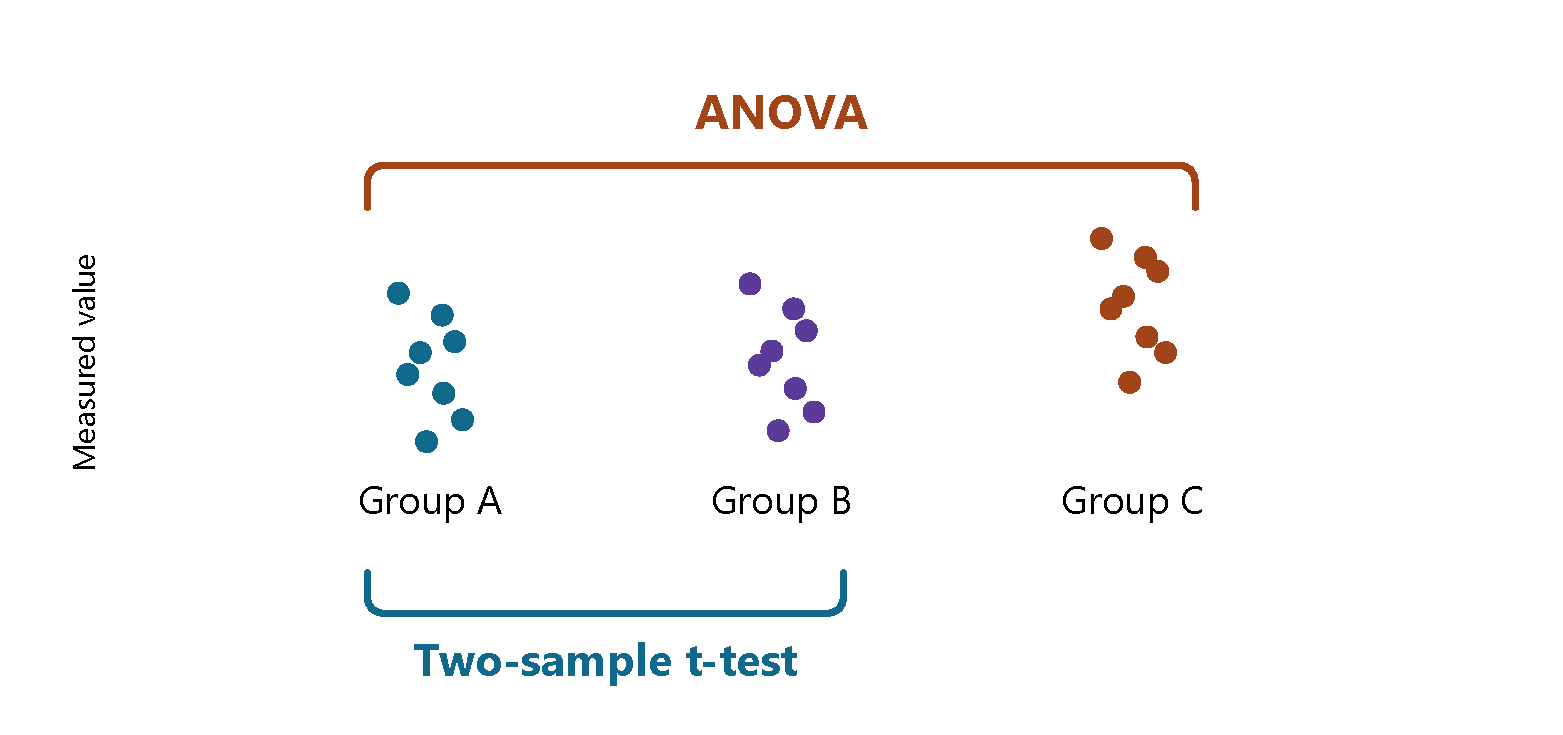
\includegraphics[width=\linewidth,height=.62\textheight,keepaspectratio]{asset-528710b91a651eb504368663af3a8178b4853315da976179567bba1821f71c59.pdf}\end{center}

\medskip

\clearpage
\section{Design and compute the one-way ANOVA}
\textbf{Preparation method} is the factor and \textbf{recovery (\%)} is the response. Each of the three methods has six independent preparations. Several measurements of one preparation estimate measurement repeatability, while independent preparations capture the variation introduced by preparation itself. The three means are 94.00\%, 98.00\% and 93.00\%, and the grand mean is 95.00\%.


Subtract the grand mean from each observation to measure total variation. The resulting decomposition assigns 84 squared percentage points to differences between method means and 30 to scatter around those means. Their sum is 114. The between-method calculation weights each squared departure from the grand mean by the number of preparations in that method.


The F ratio in \hyperref[material-7f7ee6ee0a9a140db1cbcbee21cd1bed0abeb3c6970094ce3255aa6a9b8d3d37]{Eq.~\ref*{material-7f7ee6ee0a9a140db1cbcbee21cd1bed0abeb3c6970094ce3255aa6a9b8d3d37}} compares the two mean squares in \hyperref[material-14a90c7fd0504e590bc137da9dc9e6cb8f7a70e9f96030fbcacd15ac3641c871]{Fig.~\ref*{material-14a90c7fd0504e590bc137da9dc9e6cb8f7a70e9f96030fbcacd15ac3641c871}}. Divide 84 by the two between-method degrees of freedom to get a mean square of 42. Divide 30 by the fifteen residual degrees of freedom to get 2. Their ratio is \textbf{F = 21}, with a right-tail p-value of about \textbf{0.00004484} under the equal-means null and the classical assumptions. The result points to a difference somewhere among the method means.


\par\medskip
\noindent\begin{minipage}{\linewidth}
\refstepcounter{equation}\label{material-7f7ee6ee0a9a140db1cbcbee21cd1bed0abeb3c6970094ce3255aa6a9b8d3d37}
\noindent\textbf{Eq.~\ref*{material-7f7ee6ee0a9a140db1cbcbee21cd1bed0abeb3c6970094ce3255aa6a9b8d3d37}.} The one-way F statistic compares signal to residual scatter using the two mean squares.\par\nopagebreak
\begin{center}\begin{adjustbox}{max width=\linewidth}$\displaystyle F=\frac{\mathrm{MS}_{B}}{\mathrm{MS}_{W}}$\end{adjustbox}\end{center}

\par\noindent\textbf{Symbols}

\begin{itemize}\setlength{\itemsep}{1pt}\setlength{\parsep}{0pt}
\item \textbf{F}: dimensionless omnibus test statistic.
\item \textbf{\(MS_B\)}: group-size-weighted between-group sum of squares divided by (k\ensuremath{-}1), in percentage points squared.
\item \textbf{\(MS_W\)}: residual within-group sum of squares divided by (N\ensuremath{-}k), in percentage points squared.
\item \textbf{B/W}: subscripts meaning between groups/within groups.
\item \textbf{k}: number of groups; k>1.
\item \textbf{N}: total observations; N>k.
\item \textbf{=}: equality.
\item \textbf{fraction bar}: division of \(MS_B\) by \(MS_W\).
\end{itemize}

The fixed-effects model assumes independent Normal errors with a common positive variance. The omnibus test asks whether all population means are equal. \(MS_W\) must be positive; F is undefined when this error mean square is zero.

\end{minipage}\par
\medskip

\par\medskip
\Needspace{10cm}
\refstepcounter{figure}\label{material-14a90c7fd0504e590bc137da9dc9e6cb8f7a70e9f96030fbcacd15ac3641c871}
\noindent\textbf{Fig.~\ref*{material-14a90c7fd0504e590bc137da9dc9e6cb8f7a70e9f96030fbcacd15ac3641c871}.} The completed one-way ANOVA table for the 18 river-water preparations.\par\nopagebreak
\begin{center}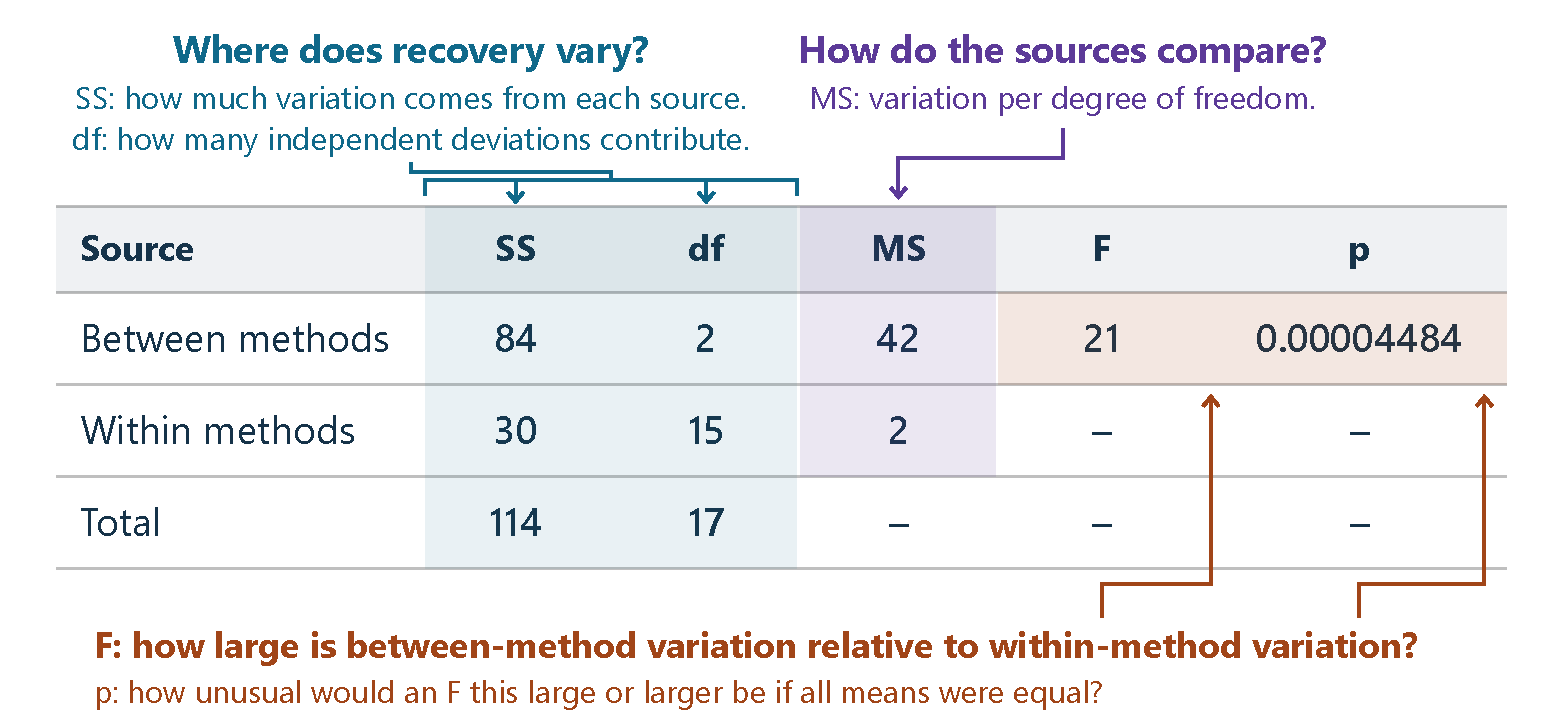
\includegraphics[width=\linewidth,height=.62\textheight,keepaspectratio]{asset-f91208827223003a97c1c62700aa52a69e7ccae87bd272be7882b22f6e6408c2.pdf}\end{center}

\medskip

\clearpage
\section{Check residuals and interpret the effect size}
A residual is observed recovery minus the fitted method mean. Classical ANOVA assumes independent errors with approximately normal distributions and common variance. Independence comes from the design. In a normal Q–Q plot, compare the ordered residuals with the reference line and look for systematic departures, including deviations at both tails. A test that estimates the normal parameters from the residuals needs calibration that accounts for fitting. The lecture illustrates this with refitting in a simulation.


The effect-size formula in \hyperref[material-f94e667e4271e95b80da79c740f8ac1b7b0abdbb746839c047b0918fd19f82cf]{Eq.~\ref*{material-f94e667e4271e95b80da79c740f8ac1b7b0abdbb746839c047b0918fd19f82cf}} relates the between-method sum of squares to the total. The one-way method effect accounts for \textbf{84 ÷ 114 = 73.7\%} of the total sum of squares in this sample. This fraction is eta squared. It describes how much of the observed variation the grouping accounts for.


\par\medskip
\noindent\begin{minipage}{\linewidth}
\refstepcounter{equation}\label{material-f94e667e4271e95b80da79c740f8ac1b7b0abdbb746839c047b0918fd19f82cf}
\noindent\textbf{Eq.~\ref*{material-f94e667e4271e95b80da79c740f8ac1b7b0abdbb746839c047b0918fd19f82cf}.} Eta squared for the preparation-method effect in the one-way ANOVA.\par\nopagebreak
\begin{center}\begin{adjustbox}{max width=\linewidth}$\displaystyle \eta^2=\frac{SS_B}{SS_T}=\frac{84}{114}\approx0.73684$\end{adjustbox}\end{center}

\par\noindent\textbf{Symbols}

\par\noindent\textbf{\ensuremath{\eta}\ensuremath{{}^2} and SS} \ensuremath{\eta}\ensuremath{{}^2} (eta squared) is the dimensionless share of observed variation attributed to the method factor. SS means sum of squared deviations; B is between methods and T is total.

\par\noindent\textbf{84 and 114} 84 is the between-method SS; 114 is total SS. Both are in squared percentage points.

\par\noindent\textbf{Operations} The fraction bars divide. The equals signs show exact equality. \ensuremath{\approx} means approximately equal after rounding to 0.73684.

\end{minipage}\par
\medskip

The regrouping exercise in \hyperref[material-1b70c5f8efa0524f7bf94560ceddd61754e49ca2b7c37cb27dc15e58586c88f1]{Fig.~\ref*{material-1b70c5f8efa0524f7bf94560ceddd61754e49ca2b7c37cb27dc15e58586c88f1}} keeps the same observations and changes the labels to hypothetical operators. The operator groups use different mixes of preparation methods. Differences between these groups therefore combine operator labels with the method mix. Comparing their raw eta squared values does not isolate an operator effect.


\par\medskip
\Needspace{10cm}
\refstepcounter{figure}\label{material-1b70c5f8efa0524f7bf94560ceddd61754e49ca2b7c37cb27dc15e58586c88f1}
\noindent\textbf{Fig.~\ref*{material-1b70c5f8efa0524f7bf94560ceddd61754e49ca2b7c37cb27dc15e58586c88f1}.} The same recovery observations grouped by method and by hypothetical operator.\par\nopagebreak
\begin{center}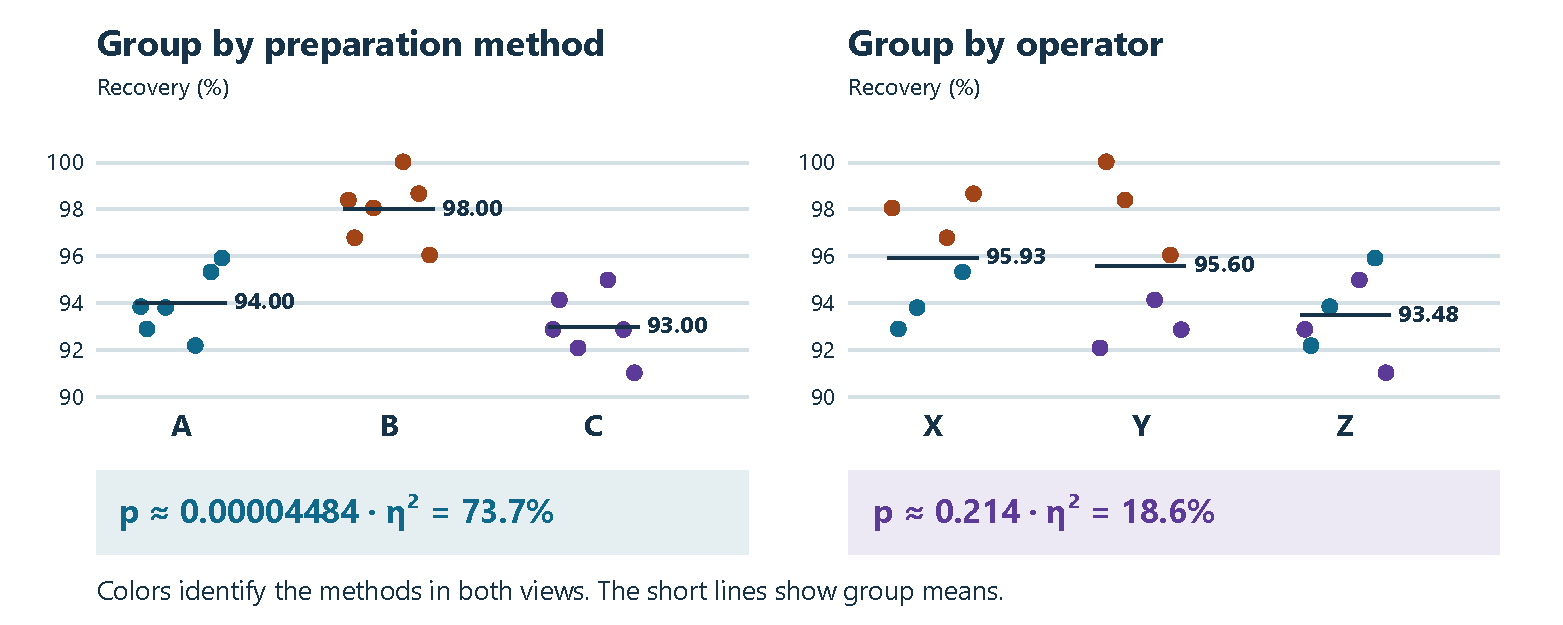
\includegraphics[width=\linewidth,height=.62\textheight,keepaspectratio]{asset-24a831f4df6b635ab69732eb7917a72c26a653a73a9c41834d97c79813b3379e.pdf}\end{center}

\medskip

\clearpage
\section{Add a second factor}
The SPE design crosses three preparation methods with two water matrices. Each combination has six independent preparations, for 36 in total. The additive model fits an overall difference between methods and an overall difference between matrices. It uses the same method differences in both matrices.


A second study crosses three treatment techniques with three water conditions: natural organic matter addition, phosphate addition and ozone pretreatment. Each combination contains four independent runs. The response is contaminant removal (\%).


Read across \hyperref[material-c64e31c106ef433644583a22cd10c21dd948ef84aa3001f30c4760fc01f03c97]{Fig.~\ref*{material-c64e31c106ef433644583a22cd10c21dd948ef84aa3001f30c4760fc01f03c97}} to see what changes as a second factor enters the analysis. The river-water method comparison is clear in the one-way analysis, while the additive comparison across both matrices gives p = 0.522. In the treatment study, the technique effect remains significant after adding the water condition. To understand these patterns, examine the mean profiles and test interaction.


\par\medskip
\Needspace{10cm}
\refstepcounter{figure}\label{material-c64e31c106ef433644583a22cd10c21dd948ef84aa3001f30c4760fc01f03c97}
\noindent\textbf{Fig.~\ref*{material-c64e31c106ef433644583a22cd10c21dd948ef84aa3001f30c4760fc01f03c97}.} One-way and additive two-way ANOVA results in the two studies.\par\nopagebreak
\begin{center}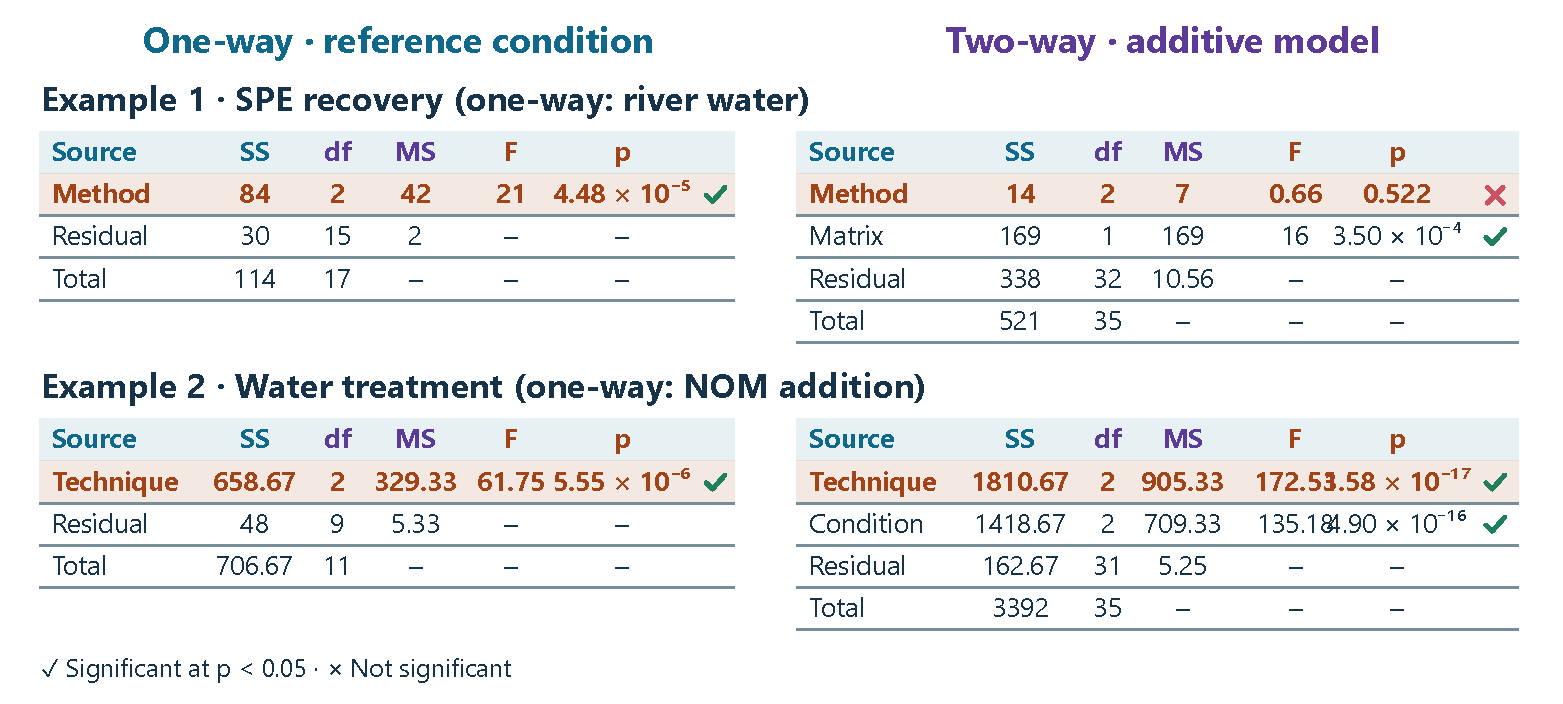
\includegraphics[width=\linewidth,height=.62\textheight,keepaspectratio]{asset-dd0dca8c1397f0232c4c51c46304ef198595b8fb5debe1231bbdc3146a59f73f.pdf}\end{center}

\medskip

\clearpage
\section{Test whether the factor effects depend on each other}
An interaction means that the difference between levels of one factor changes across levels of another. For the SPE data, method B exceeds method A by 4.00 percentage points in river water and falls below it by 6.00 points in wastewater. The direction reverses. The treatment profiles are closer to parallel, so the difference between techniques is more stable across conditions. In the balanced design, \hyperref[material-c9f3b6340d5814eb17871da456d0a7b2583b561b01450bd0c72be7143c97f358]{Eq.~\ref*{material-c9f3b6340d5814eb17871da456d0a7b2583b561b01450bd0c72be7143c97f358}} shows how to turn those departures from the additive pattern into a sum of squares.


\par\medskip
\noindent\begin{minipage}{\linewidth}
\refstepcounter{equation}\label{material-c9f3b6340d5814eb17871da456d0a7b2583b561b01450bd0c72be7143c97f358}
\noindent\textbf{Eq.~\ref*{material-c9f3b6340d5814eb17871da456d0a7b2583b561b01450bd0c72be7143c97f358}.} Interaction gaps, their contribution to the sum of squares, and the resulting variance partition.\par\nopagebreak
\begin{center}\begin{adjustbox}{max width=\linewidth}$\displaystyle \begin{aligned}
\bar y_{ij\cdot}&=\frac{1}{r}\sum_{k=1}^{r}y_{ijk}\\
d_{ij}&=\underbrace{\bar y_{ij\cdot}}_{\text{mean for the combination}}-\underbrace{\Bigl(\overbrace{\bar y_{i\cdot\cdot}}^{\text{factor A mean}}+\overbrace{\bar y_{\cdot j\cdot}}^{\text{factor B mean}}-\overbrace{\bar y_{\cdot\cdot\cdot}}^{\text{grand mean}}\Bigr)}_{\text{reference from the factor means}}\\
SS_{AB}&=r\sum_{i=1}^{a}\sum_{j=1}^{b}d_{ij}^{2}=SS_{\mathrm{res,add}}-SS_W\\
SS_T&=SS_A+SS_B+SS_{AB}+SS_W
\\r&=\frac{N}{ab},\qquad \text{SPE: }r=\frac{36}{3\times 2}=6
\end{aligned}$\end{adjustbox}\end{center}

\par\noindent\textbf{Symbols}

\begin{itemize}\setlength{\itemsep}{1pt}\setlength{\parsep}{0pt}
\item \textbf{\(i\), \(j\)}: Levels of factors A and B that identify a combination.
\item \textbf{\(\bar y_{ij\cdot}\)}: Observed mean for one combination. \(y_{ijk}\) is recovery for preparation \(k\) in that combination. A bar denotes a mean and a dot pools the corresponding index.
\item \textbf{\(\bar y_{i\cdot\cdot}\), \(\bar y_{\cdot j\cdot}\)}: Means across all runs at the indicated level of A or B.
\item \textbf{\(\bar y_{\cdot\cdot\cdot}\)}: Overall mean of all runs. The means are expressed in percent.
\item \textbf{\(d_{ij}\)}: Gap between the observed mean and its reference from the factor means, in percentage points.
\item \textbf{\(a\), \(b\)}: Numbers of levels of factors A and B, respectively.
\item \textbf{\(r\)}: Number of independent runs per combination. Each combination has the same run count. In the SPE example, \(r=6\).
\item \textbf{\(N\)}: Total number of independent runs across all \(ab\) combinations. Divide by \(ab\) to get \(r\).
\item \textbf{\(SS_T\), \(SS_A\), \(SS_B\)}: Total sum of squares and sums of squares for the two factors.
\item \textbf{\(SS_{AB}\), \(SS_W\)}: Interaction sum of squares and remaining residual sum of squares. \(SS_{\mathrm{res,add}}\) is the residual sum of squares in the additive model. All sums of squares are in squared percentage points.
\item \textbf{\(\sum\), \(+,-,=,{}^2\)}: Add across the indicated levels, add, subtract, equality and square. The multiplier \(r\) weights each squared gap by its run count.
\end{itemize}

The formulas use a balanced design with the same number of runs for every combination.

\end{minipage}\par
\medskip

For each method and matrix combination, the additive reference is its method mean plus its matrix mean minus the grand mean. For method B in river water these three values are 92.00\%, 95.00\% and 92.83\%. The resulting reference is 94.17\% and the observed mean is 98.00\%. The interaction gap is about +3.83 percentage points. Square the unrounded gap and multiply by the six independent preparations to get this combination’s contribution, about 88.17 squared percentage points. Repeat for all six combinations and add the contributions.


In \hyperref[material-3c315c1673350b82fd25dcc057e7d1aa4842f414d7a495ce8043e9563c112a68]{Fig.~\ref*{material-3c315c1673350b82fd25dcc057e7d1aa4842f414d7a495ce8043e9563c112a68}}, adding the interaction assigns 278 of the additive residual sum of squares of 338 to the interaction and leaves 60. The overall sum of squares stays at 521. In this balanced design the method sum of squares also stays fixed. Its p-value drops to 0.043 as the residual mean square decreases, while its eta squared remains 2.69\%. The interaction accounts for 53.36\% of the total variation. For treatment, the interaction accounts for 0.79\% and gives p = 0.287. The 1\%, 6\% and 14\% marks are Cohen’s rough benchmarks as discussed by Lakens (2013). Practical importance depends on which recovery differences matter for the application.


\par\medskip
\Needspace{10cm}
\refstepcounter{figure}\label{material-3c315c1673350b82fd25dcc057e7d1aa4842f414d7a495ce8043e9563c112a68}
\noindent\textbf{Fig.~\ref*{material-3c315c1673350b82fd25dcc057e7d1aa4842f414d7a495ce8043e9563c112a68}.} Interaction tests, effect sizes and the comparison with the additive residual.\par\nopagebreak
\begin{center}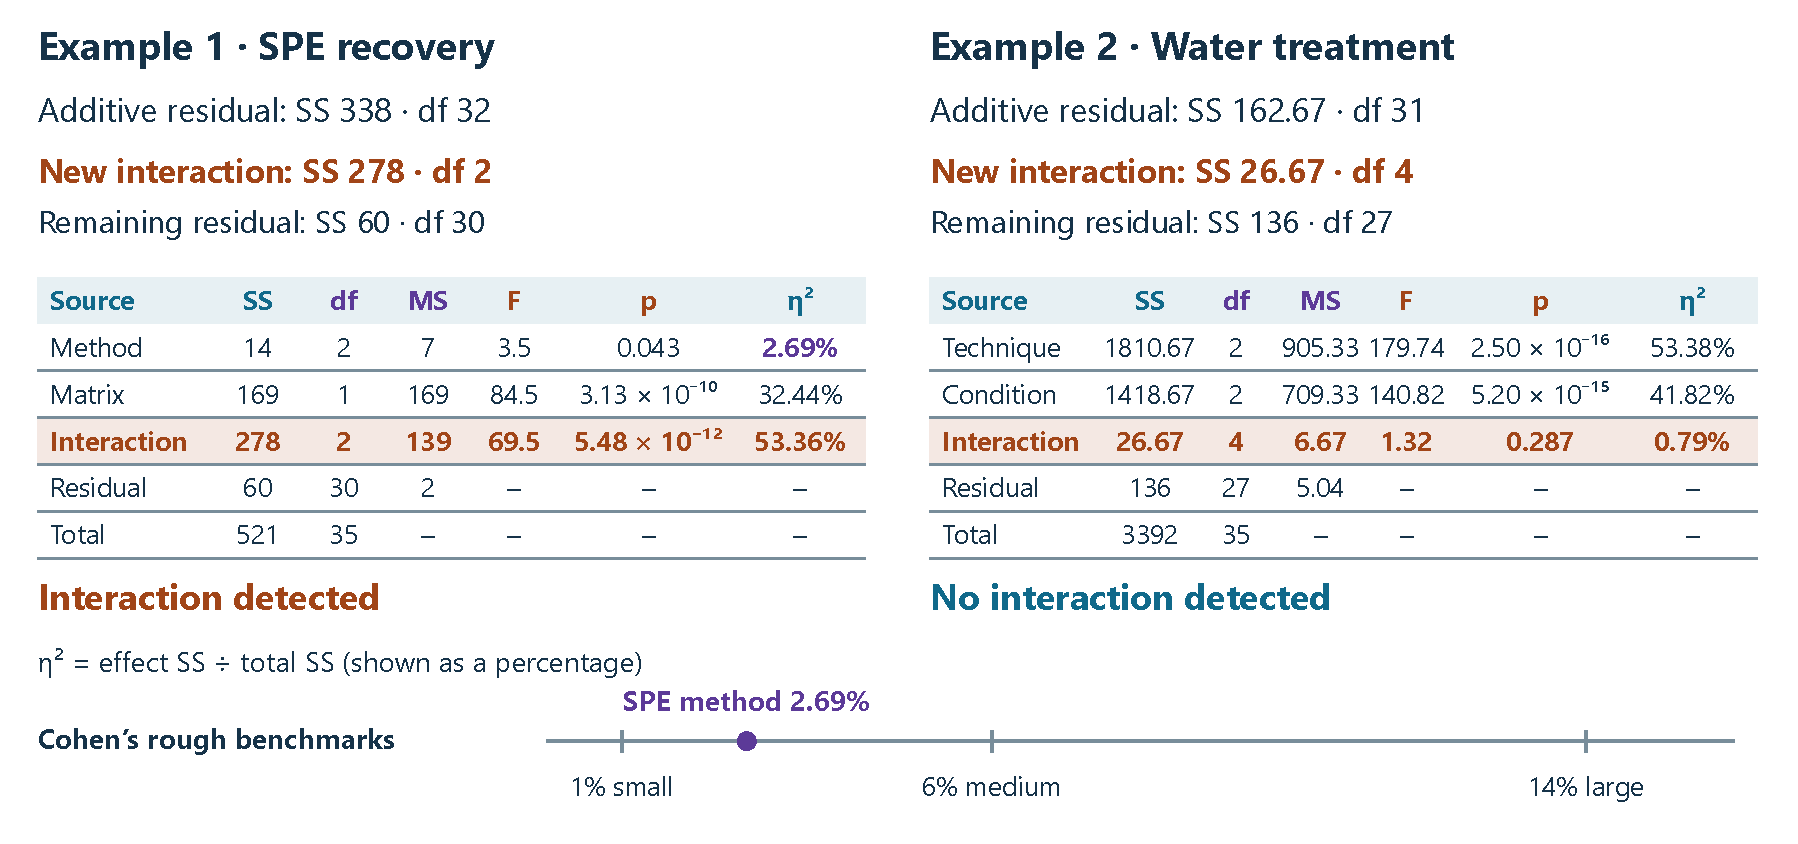
\includegraphics[width=\linewidth,height=.62\textheight,keepaspectratio]{asset-d0ca8ca84cab5e4f495d45e78edc62e1e80646fac384c274dd04b1cbdd186d9a.pdf}\end{center}

\medskip

\clearpage
\section{Locate differences with Tukey HSD}
Tukey HSD compares all pairs of group means within a specified family. For equally sized groups, use \hyperref[material-27fd5a61e08ad650319aacc35f590212f41068d7825db61a2e883b7895f4601f]{Eq.~\ref*{material-27fd5a61e08ad650319aacc35f590212f41068d7825db61a2e883b7895f4601f}}. Multiply the critical studentized range value by the square root of the ANOVA residual mean square divided by the number of observations per group. The studentized range is the spread from the smallest to the largest group mean under the equal-means null, scaled by the estimated standard error of one mean. The cutoff depends on the family’s number of groups, the residual degrees of freedom and the chosen error rate.


\par\medskip
\noindent\begin{minipage}{\linewidth}
\refstepcounter{equation}\label{material-27fd5a61e08ad650319aacc35f590212f41068d7825db61a2e883b7895f4601f}
\noindent\textbf{Eq.~\ref*{material-27fd5a61e08ad650319aacc35f590212f41068d7825db61a2e883b7895f4601f}.} Tukey’s critical mean difference for equal group sizes.\par\nopagebreak
\begin{center}\begin{adjustbox}{max width=\linewidth}$\displaystyle \mathrm{HSD}=q_{\mathrm{crit}}\sqrt{\frac{\mathrm{MS}_E}{n}}$\end{adjustbox}\end{center}

\par\noindent\textbf{Symbols}

\begin{itemize}\setlength{\itemsep}{1pt}\setlength{\parsep}{0pt}
\item \textbf{\(HSD\)}: The minimum absolute difference for significance, in the same units as the response.
\item \textbf{\(q_{crit}\)}: The dimensionless upper critical value of the studentized range for the number of group means, the residual degrees of freedom, and the chosen familywise significance level.
\item \textbf{\(MS_E\)}: The residual mean square from ANOVA, in squared response units.
\item \textbf{\(n\)}: The common number of independent observations per group.
\item \textbf{Operations}: The fraction divides the residual mean square by the group size. The square root restores the response units and multiplication by the critical value gives the cutoff.
\end{itemize}

\end{minipage}\par
\medskip

Take three methods with means of 10, 12 and 17 mg/L, five observations each and a residual mean square of 4 squared mg/L. At the 5\% level, the reference table gives 3.77 for three groups and 12 residual degrees of freedom. The HSD is 3.37 mg/L. The gaps of 7 and 5 mg/L exceed this threshold. The gap of 2 mg/L leaves the A–B comparison inconclusive.


In \hyperref[material-cdee98ea0f7f9c6aa6236f56a6342ddadfdaaeed82ab5dfca8ef30a3e737d0c7]{Fig.~\ref*{material-cdee98ea0f7f9c6aa6236f56a6342ddadfdaaeed82ab5dfca8ef30a3e737d0c7}}, each water matrix has its own Tukey family of three method comparisons, using the residual mean square of the full SPE model. The matrix gives adjusted p-values and the plot shows signed differences with simultaneous 95\% intervals within each matrix. Intervals excluding zero identify significant comparisons. Method B differs from both A and C in each matrix, with the direction reversed. The A–C intervals include zero in both matrices.


\par\medskip
\Needspace{10cm}
\refstepcounter{figure}\label{material-cdee98ea0f7f9c6aa6236f56a6342ddadfdaaeed82ab5dfca8ef30a3e737d0c7}
\noindent\textbf{Fig.~\ref*{material-cdee98ea0f7f9c6aa6236f56a6342ddadfdaaeed82ab5dfca8ef30a3e737d0c7}.} Adjusted p-values and Tukey intervals for the SPE method comparisons.\par\nopagebreak
\begin{center}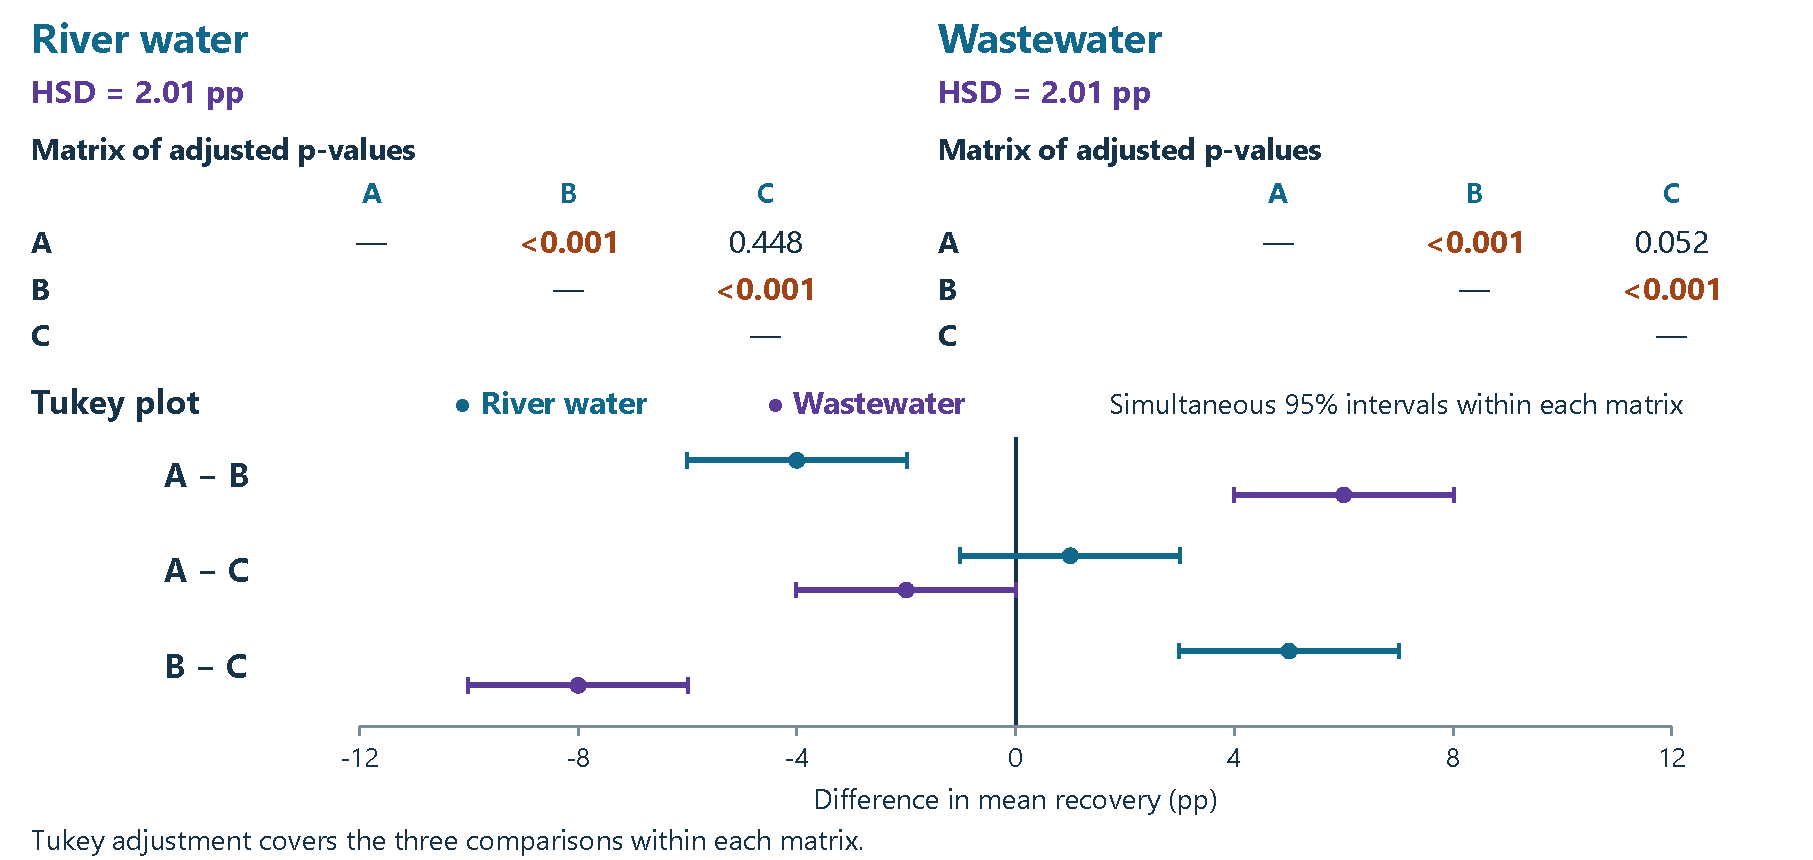
\includegraphics[width=\linewidth,height=.62\textheight,keepaspectratio]{asset-64077675a0aa666922d74d703b7401243daa600677fd1fcd3827241054f1bd94.pdf}\end{center}

\medskip

\end{document}
